\section{Darstellung der methodischen Vorgehensweise}\label{sec:methode}
Die Vorgehensweise für die Entwicklung des Geschäftsprozesses orientiert sich an der den Vorgehensmodellen zur Softwareentwicklung (siehe Abschnitt \ref{sec:methodenGrundlage}) und an den existierenden Forschungsansätze dynamischer Geschäftsprozesse auf Basis von Ereignisverarbeitung (siehe Abschnitt \ref{sec:Kombi}). 
In Abbildung \ref{fig:Vorgehensweise in der Übersicht} wird die methodischen Vorgehensweise in der Übersicht dargestellt.  

Im Forschungsansatz [moby]\textsuperscript{dbpm} wird von \citeauthor{Vidackovic.2014} ein ähnliches Vorgehen zur Entwicklung dynamischer Geschäftsprozesse dargelegt. Fachlich ähnelt sich das Ziel, trotz
des Themenschwerpunkts der modellbasierten Softwareentwicklung und dem Unterschied das kein Anwendungsfall konkretisiert wird, dem dieser Bachelorarbeit. \cite{Vidackovic.2014}
Daher orientiert sich diese Bachelorarbeit grundlegend an seinem Vorgehen. Es handelt sich bei der Dissertation um einen wissenschaftlichen Aufsatz der Schriftenreihe zu Arbeitswissenschaft und Technologiemanagement des Fraunhofer-Institut für Arbeitswirtschaft und Organisation und damit um wissenschaftlich valides Wissen.

\begin{figure}[H]
	\centering 
    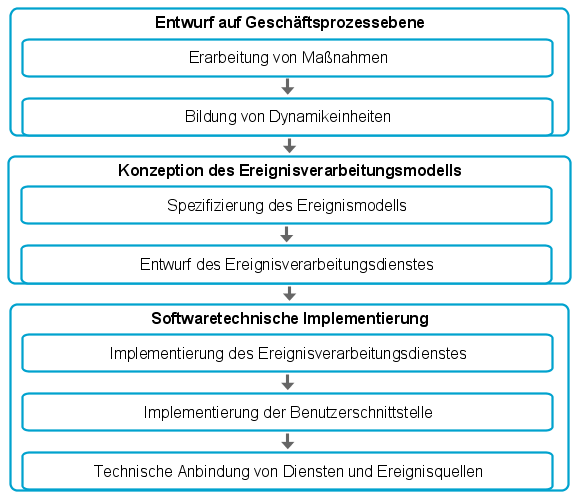
\includegraphics[width=\textwidth]{img/methode.png}	
    \caption[Vorgehensweise in der Übersicht]
    {Vorgehensweise in der Übersicht\protect\footnotemark}
    \label{fig:Vorgehensweise in der Übersicht}
\end{figure}
\footnotetext{Eigene Darstellung}
\footnotetext{Die Abbildung dient lediglich der Visualisierung und ist nicht \ac{BPMN} 2.0 konform.}

\newpage

Zuerst werden anhand der Prinzipien von Lean Management sowie der Erkenntnisse aus den Experteninterviews geeignete Maßnahmen definiert, die zur Dynamisierung der Fertigungsdurchführung beitragen.
Im Anschluss werden diese mit dynamischen Eigenschaften versehen, indem aus den Aktivitäten der Fertiungsdurchführung sogenannte Dynamikeinheiten (siehe Abchnitt \ref{sec:Kombi}) in Wechselwirkung mit Ereignissen gebildet werden. Hier werden demnach insbesondere die Ereignisse modelliert, die während der Durchführung des Geschäftsprozesses mit der Ereignisverarbeitungsebene ausgetauscht werden.

Bei der anschließenden Konzeption auf Ereignisverarbeitungsebene  wird das notwendige Ereignismodell spezifizert und das Regelwerk der Ereignisverarbeitung definiert. Das Ereignismodell umfasst hierbei auch die einzelnen Ereignisobjekte. Diese stellen jene Ereignisse dar, welche in Wechselwirkung mit SAP S/4HANA Cloud ausgetauscht werden. Nachfolgend wird das Geschäftsprozessmodell komplettiert und dargestellt.

Im letzten Schritt erfolgt schließlich die softwaretechnische Implementierung. Hierfür wird der Ereignisverarbeitungsdienst in eine ausführbare Programmiersprache übersetzt und eine Benutzerschnittstelle zur Interaktion mit dem Anwender entwickelt. Andererseits wird auch die technische Integration mit SAP S/4HANA Cloud und anderen notwendigen Diensten durchgeführt 